\section{Morse-Homologie ist zelluläre Homologie}

Das Ziel dieses Abschnittes ist es, mithilfe der im 2. Kapitel erarbeiteten Mitteln eine 
CW-Zerlegung von einer kompakten Mannigfaltigkeit $M$ zu finden.

Wir kennen schon eine disjunkte Zerlegung von $M$ in offene Kreisscheiben, nämlich
\[ \mathcal{E} = \{ \unst (p): p \in \Crit (f) \} . \]
Tatsächlich ist jede instabile Mannigfaltigkeit eine offene Kreisscheibe und jeder Punkt in 
$ p \in M$ wird von $\phi_{\bullet}(p)$ für $t \to - \infty$ genau auf einen kritischen Punkt 
transportiert (siehe Prop.~\ref{prop: trajektorien enden in kritischen punkten}), also ist 
$\mathcal{E}$ eine disjunkte Überdeckung.

\begin{prop}
    \label{prop: cw-zerlegung}
    Die Zerlegung $\mathcal{E} = \{ \unst (p): p \in \Crit (f) \}$ ist eine CW-Zerlegung.
\end{prop}

Bevor wir diese Proposition beweisen können, müssen wir noch ein wenig arbeiten.
Wir definieren für einen kritischen Punkt $p$:
\[ \clunst (p) = 
    \unst (p) \cup \left( \bigcup_{q \in \Crit (f)} \Lb (p, q) \times \unst (q) \right) . \]

$\Lb (p, q) \times \unst (q)$ ist nur nicht leer, wenn $\Index (p) > \Index (q)$.
Für alle $x \in \unst (p) - \{ p \}$ gibt es einen kritischen Punkt $q$ und eine Trajektorie 
$\lambda_x \in \Lt (p, q)$, sodass $x \in \lambda_x$. wir können also jedes 
$x \in \unst (p) - \{ p \}$ künstlich zu einem Tupel $(\lambda_x, x)$ machen. Wir werden im Folgenden
nicht zwischen $x$ und $(\lambda_x, x)$ in $\unst (p)$ unterscheiden.

Wie im letzten Kapitel geben wir für $\clunst (p)$ eine Topologie:

\begin{definition}[Topologie von $\clunst (p)$]
    Wir definieren eine Basis der Topologie von $\clunst (p)$. Offene Mengen in $\unst (p)$ sind 
    auch in $\clunst (p)$ offen. Für $(\lambda, x) \in \Lt (p, c_1) \times \Lt (c_{k - 1}, c)$,
    eine Umgebung $U^0$ von $x$ in $M$ und $U^+$ und $U^-$ wie vorher 
    in~\ref{def: topologie gebrochener trajektorien} die Vereinigungen offener Umgebungen der Ein-
    bzw. Austrittspunkte der jeweiligen Trajektorien in $\del_+ \Omega (c_i)$ bzw. 
    $\del_- \Omega (c_i)$ definieren wir die restlichen Elemente 
    $\mathcal{U}(\lambda, x, U^0, U^-, U^+)$ der Basis
    wie folgt: \\
    Falls $(\mu, x') \in \Lb(p, c_i) \times \unst (c_i)$ oder $(\mu, x') \in W^u (p) \cap \stab (c)$, 
    dann ist \[ (\mu, x') \in \mathcal{U}(x, \lambda, U^0, U^-, U^+) , \]
    falls gelten:
    \begin{enumerate}
        \item $x' \in U^0$.
        \item Die (einfache) Trajektorie, die $c_i$ mit $x'$ verbindet, tritt in $\Omega (c_j)$ durch 
            $U^+_j$ für alle $j > i$ und verlässt $\Omega (c_j)$ durch $U^-_j$ für alle $j \geq i$.
            Eine solche Trajektorie existiert, da $x' \in \unst (c_i)$.
        \item $\mu \in \mathcal{U}(\tilde{\lambda}, \tilde{U}^-, \tilde{U}^+)$, wobei 
            $\tilde{\lambda} = (\lambda_1, \dots, \lambda_i)$ und 
            $\tilde{U}^{\pm} = \bigcup_{j = 1}^i U^{\pm}_j$
    \end{enumerate}
    Für $(\mu, x) \in \unst(p) \cap \stab (c)$ sind die zweite und die dritte Bedingung äquivalent.
    Die offenen Mengen in $\clunst (p)$ sind dann die Mengen, die sich als Vereinigung der 
    Elemente der Basis schreiben lassen. 
\end{definition}

\begin{example}
    \begin{itemize}
        \item Die Höhenfunktion $f$ von $S^2 \subseteq \R^3$ ist eine Morse Funktion. Diese hat 
            zwei kritische Punkte: den Nordpol $n$ und den Südpol $s$. Es gilt 
            $\unst (n) = S^2 - \{ s \}$ und $\unst (s) = \{ s \}$. $\Lb (n, s) = \Lt (n, s) = S^1$,
            und dann ist $\clunst (n)$ die abgeschlossene Kreisscheibe mit Rand $\Lt (n, s)$. 
        \item Wir betrachten den kritischen Punkt $p$:
            \begin{figure}[H]
                \centering
                \begin{tikzpicture}
                    % Include the image in a node
                    \node [
                        above right,
                        inner sep=0] (image) at (0,0) {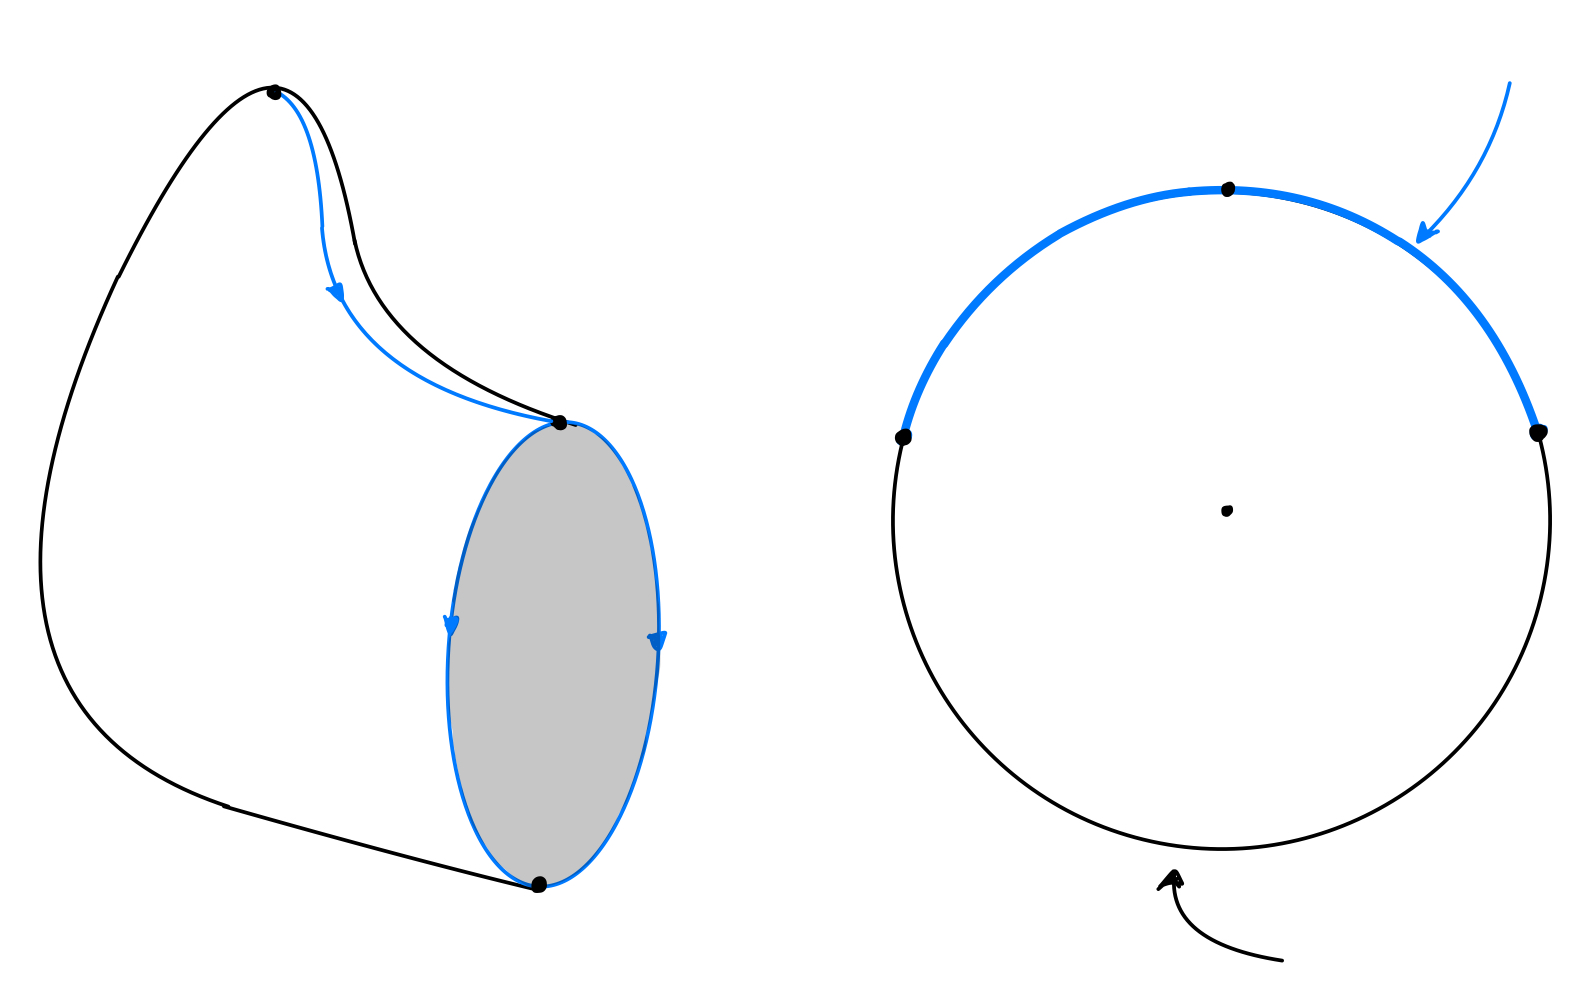
\includegraphics[width=0.4\textwidth]{../resources/clunst-beispiel.jpeg}};
                        
                    % Create scope with normalized axes
                    \begin{scope}[
                    x={($0.05*(image.south east)$)},
                    y={($0.1*(image.north west)$)}]

                    % Annotate left figure
                    \node at (3.5, 9.5) {\tiny $p$};
                    \node at (7, 6.2) {\tiny $c$};
                    \node at (7, 0.6) {\tiny $q$};
                    
                    \node[text=LightBlue] at (4.2, 6.2) {\tiny $\ell$};
                    \node[text=LightBlue] at (5, 3.8) {\tiny $\ell_1$};
                    \node[text=LightBlue] at (9, 3.8) {\tiny $\ell_2$};

                    % Annotaste right figure
                    \node at (15.5, 4.5) {\tiny $p$};
                    \node at (15.5, 8.5) {\tiny $(\ell, c)$};

                    \node at (13.3, 5.6) {\tiny $((\ell, \ell_1), q)$};
                    \node[right] at (19.1, 5.6) {\tiny $((\ell, \ell_1), q)$};

                    \node at (19, 0.5) {\tiny $\Lb (p, q) \times \{ q \}$};
                    \node[text=LightBlue] at (19, 9.5) {\tiny $\{ \ell \} \times \unst (c)$};

                    % \draw[lightgray,step=1] (image.south west) grid (image.north east);
                    \end{scope}
                \end{tikzpicture}
            \end{figure}
    \end{itemize}
\end{example}

\begin{prop}
    \label{prop: abschluss von instabilen mannigfaltigkeiten}
    Ist $p$ ein kritischer Punkt von $f$, $k = \Index (p)$, dann ist $\clunst (p)$ homeomorph 
    zur abgeschlossenen Kreisscheibe $D^k$, und $\unst (p)$ ist das Innere von $\clunst (p)$.
\end{prop}

\begin{remark}
    Mit dieser Proposition wird auch Proposition~\ref{prop: cw-zerlegung} bewiesen:
    Die ersten beiden Bedingungen für CW-Zerlegungen sind schon erfüllt. Da wir annehmen, dass 
    $M$ kompakt ist, sind auch die letzten beiden Bedingungen erfüllt. Die dritte Bedingung folgt
    dann sofort aus der letzten Proposition~\ref{prop: abschluss von instabilen mannigfaltigkeiten}.
\end{remark}

\begin{bigproof}
    Wir geben nur eine grobe Beweisidee. Den detaillierten Beweis findet man in \cite{audin}.
    Für Elemete $(\lambda, x) \in \clunst (p)$ gilt sobieso schon, dass $f(x) \leq f(p)$. Definiere
    \[ \clunst (p, \alpha) = 
        \{ (\lambda, x) \in \clunst (p) - \{ p \} : f(x) \geq \alpha \}  \cup \{ p \} . \]
    Für $\alpha = f(c) - \eps$ und $\eps$ klein genug gilt 
    \[ \clunst (p, \alpha) = \unst (p) \cap \Omega (p, \eps, \eta) . \]
    Für ein belibiges $\eta$. $\Omega (p, \eps, \eta)$ ist wie in der Notation zu 
    Morse-Umgebungen~\ref{def: notation morse umgebung}. Dies ist via einer Morse-Karte homeomorph 
    zu $V^- \cap U(\eps, \eta)$, also zur abgeschlossenen $\Index (p)$-dimensionalen Kreisscheibe.
    Da $M$ kompakt ist besitzt $f$ ein Minimum, und falls gilt $\alpha < \min (f)$, dann gilt 
    offenbar
    \[ \clunst (p, \alpha) = \clunst (p) . \]
    Wir wollen also zeigen, dass für $\alpha' < \alpha$ gilt
    \[ \clunst (p, \alpha') \isom \clunst (p, \alpha) . \]
    Die Menge $\clunst (p, \alpha)$ erinnert uns an die Subniveaumengen aus 
    Abschnitt~\ref{sec: topologische eigenschaften anhand kritischer punkte}. Das erste 
    Deformationslemma liefert eine ähnliche Aussage, und wir können die folgende Behauptung 
    beweisen:

    \begin{claim}
        Wenn sich im Intervall $[\alpha', \alpha]$ keine kritischen Werte von $f$
        befinden, dann sind $\clunst (p, \alpha')$ und $\clunst (p, \alpha)$ homeomorph.
    \end{claim}

    \begin{smallproof}
        Unter Anwendung des ersten Deformationslemmas auf $-f$ bekommen wir einen Homeomorphismus
        \[ \phi \colon M^{\alpha'} \longto M^{\alpha} . \]
        Die Subniveaumengen sind die Subniveaumengen von $-f$. Dann ist auch 
        \begin{align*}
            \chi \colon \clunst (p, \alpha') \longto & \clunst (p, \alpha) \\
            (\lambda, x) \longmapsto & (\lambda, \phi(x))
        \end{align*}
        ein Homeomorphismus.
    \end{smallproof}

    Sehr viel schwieriger ist es zu beweisen, dass sich $\clunst (p, \alpha)$ selbst wenn $\alpha$
    einen kritischen Wert überquert nicht verändert. Für den Fall $\Index (p) = \Index (q) + 1$
    und $\Index (q) \neq 0$ liefert die folgende Skizze eine Idee für den Beweis:

    \begin{figure}[H]
        \label{fig: definition von chi}
        \centering
        \begin{tikzpicture}
            % Include the image in a node
            \node [
                above right,
                inner sep=0] (image) at (0,0) {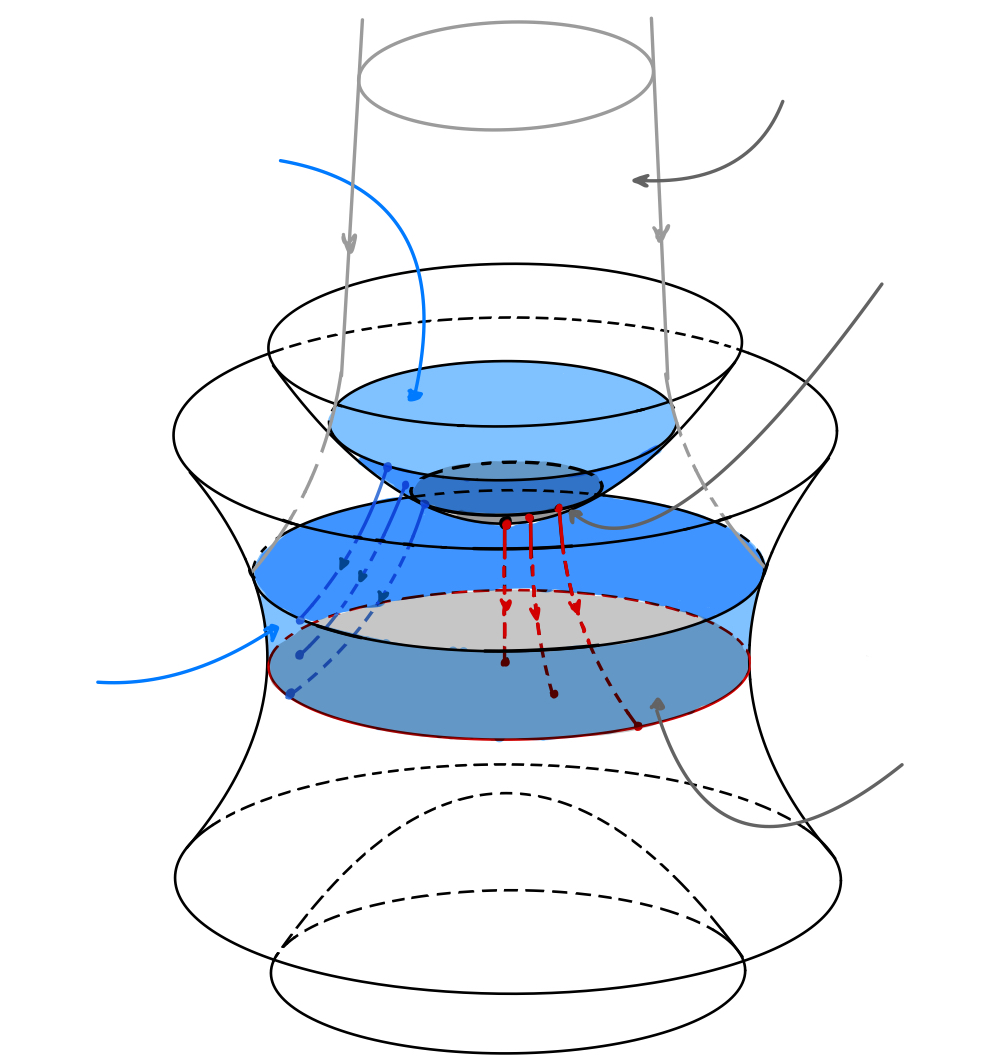
\includegraphics[width=0.4\textwidth]{../resources/cw-zerlegung.jpeg}};
                
            % Create scope with normalized axes
            \begin{scope}[
            x={($0.05*(image.south east)$)},
            y={($0.05*(image.north west)$)}]

            \node[text=LightBlue] at (0, 7) {\small $\Ima (\Phi)$};
            \node[text=DarkGray] at (22, 6.4) {\small $\unst (c) \cap f^{-1}[\alpha - \eps, \infty)$};
            \node[text=DarkGray] at (18.5, 15.2) {\small $B'$};
            \node[text=LightBlue] at (3.5, 17) {\small $B - B'$};
            \node[text=DarkGray] at (15.7, 18.8) {\small $U$};

            % \draw[lightgray,step=1] (image.south west) grid (image.north east);
            \end{scope}
        \end{tikzpicture}
        \caption{Definition von $\chi$}
    \end{figure}
    
    Wir nehmen an, dass es für jeden kritischen Wert $\alpha$ genau einen kritischen Punkt $c$ gibt, 
    sodass $f (c) = \alpha$. Es sei $c$ ein weiterer kritischer Punkt mit $f(c) = \alpha$. Dann sei $\eps > 0$, 
    sodass sich im Intervall $f^{-1}[\alpha - \eps, \alpha + \eps]$ keine kritischen Punkte außer $c$ befinden.
    Wir bekommen in diesem Fall nur ein Problem, wenn wir einen Punkt $x$ haben, der von seiner Trajektorie 
    auf den kritischen Punkt $c$ geschickt wird - ansonsten können wir wie im Beweis von Behauptung 1
    den Punkt $x$ entlang seiner Trajektorie entlang des (skalierten) Pseudo-Gradientenfeldes nach unten ziehen. 
    Wir definieren also
    \[ P = \{ (x, \lambda) \in \clunst (p, \alpha + \eps) : x \in \unst (c) \} . \]
    Außerhalb von einer Umgebung von $P$ können wir 
    \[ \chi \colon \clunst (p, \alpha + \eps) \longto \clunst (p, \alpha - \eps) \]
    wie in Behauptung 1 angedeutet definieren.

   Wir zeigen dies nur für den einfachsten Fall:

    \begin{claim}
        Ist $\alpha = f(p)$, $q$ ein weiterer kritischer Punkt von $f$ mit 
        $\Index (p) = \Index (q) + 1 \neq 0$ und $\eps > 0$ klein genug, dann sind 
        $\clunst (p, \alpha + \eps)$ und $\clunst (p, \alpha - \eps)$ homeomorph.
    \end{claim}

    \begin{smallproof}
        In diesem Fall gilt 
        \[ P \subseteq \mathcal{M} (p, c) \subseteq \unst (p) \subseteq \clunst (p) \]
        Der Beweis erinnert an den Beweis von Satz~\ref{satz: gebrochene trajektorien sind 1-dim mannigfaltigkeit}.
        Man betrachte die Folgende Abbildung:

        Da der Index sich nur um $1$ unterscheidet ist $\Lb (p, c) = \Lt (p, c)$ eine endliche Ansammlung 
        von Trajektorien. Für jede dieser Trajektorien $\ell$ wähle eine Umgebung wie in 
        Fig.~\ref{fig: definition von chi} angedeutet:

        Die Umgebung von $P$ ist an den Seiten von den äußeren Trajektorien begrenzt und oben und unten von den
        Niveaumengen $f^{-1}(\alpha + \eps + \delta)$ und $f^{-1}(\alpha - \eps)$. Wir finden wie im Beweis 
        von Satz~\ref{satz: gebrochene trajektorien sind 1-dim mannigfaltigkeit} eine Kreisscheibe 
        $B \subseteq f^{-1}(\alpha + \eps) \cap \unst (p)$, die transversal zu $S_+(c)$ ist, vollständig in der 
        gewählten Umgebung von $P$ enthalten ist und eine Umgebung vom Schnittpunkt 
        $\ell \cap f^{-1}(\alpha + \eps)$ ist. Die existenz solcher Umgebungen transversal zu $S_+(c)$ folgt 
        aus der Smale-Bedingung. Außerdem wählen wir eine weitere kleinere Kreisscheibe $B'$, 
        die die selben Eigenschaften wie $B$ und sodass gilt $B' \subsetneq B$. 

        Die graue Scheibe in der Mitte vom Bild ist $\unst (c) \cap f^{-1} [\alpha - \eps, \infty)$. 
        Wir identifizieren diese Kreisscheibe mit 
        \[ \{ \ell \} \times \unst (c) \cap f^{-1} [\alpha - \eps, \infty) \subseteq 
            \clunst (c, \alpha - \eps) . \]
        Wenn wir unsere Umgebung nun entlang der angedeuteten Pfeile ähnlich wie im Beweis 
        von~\ref{satz: erstes deformationslemma} \say{nach unten ziehen}, sodass 
        $B - B'$ auf den gefärbten Zylinderabschnitt $\Ima (\Phi)$ und $B'$ auf die mittlere Kreisscheibe 
        abgebildet wird. $\Phi$ ist wie im Beweis 
        von~\ref{satz: gebrochene trajektorien sind 1-dim mannigfaltigkeit}. 
        Es ist möglich diese Abbildung so zu wählen, dass sie am Rand der Umgebung der 
        oben gewählten Abbildung einspricht und dass es ein Homeomorphismus ist.
    \end{smallproof}

    Für einen beliebigen kritischen Punkt $c$ funktioniert der Beweis ähnlich.
\end{bigproof}

\begin{theorem}[Morse-Homologie ist zelluläre Homologie]
    \label{satz: morse-homologie ist zellulaere homologie}
    Es existiert eine Isomrphie von Kettenkomplexen zwischen dem zelluläre Kettenkomplex 
    $(C^{Cell}(X, \mathcal{E})_{\ast}, \del)$, der durch die CW-Zerlegung in instabilen 
    Mannigfaltigkeiten durch 
    Proposition~\ref{prop: cw-zerlegung} gegeben ist, und dem Morse-Komplex 
    $(C_{\ast}(M, (f, X)), \del_X)$.
\end{theorem}

\begin{proof}
    Es sei $F \colon C_k (M, (f, X)) \to C^{Cell}(X, \mathcal{E})$ die lineare Abbildung, 
    die den kritischen Punkt $p$
    auf die Zelle $\unst (p)$ schickt. Dann bildet $F$ Erzeuger auf Erzeuger ab, ist also 
    offensichtlich ein linearer Isomorphismus. Wir wollen zeigen, dass 
    $F \circ \del_X = \del \circ F$. Wir zeigen sogar, dass für kritische Punkte $p$ und $q$ mit 
    Index $k$ und $k - 1$ die Zahl $N (\unst (p), \unst (q))$, also der Grad der Abbildung 
    $\psi_{\unst (q)} \circ \phi_{\unst (p)}$ modulo $2$ gleich der Zahl $n_X(p, q)$, also 
    der Anzahl der Trajektorien von $p$ nach $q$ modulo $2$ ist. 

    Da $\Lt (p, q)$ $0$-dimensional ist, gilt $\Lb (p, q) = \Lt (p, q)$ und dann befinden sich im 
    Rand von $\clunst (p)$, also 
    \[ \bigcup_{c \in \Crit (f)} \Lb (p, c) \times \unst (c) \isom S^{k - 1} , \] 
    genau $\# \Lt (p, q)$ disjunkte Kopien von $\unst (q) \isom B^{k - 1}$. Jede dieser Kopien 
    wird mit der Anbringungsabbildung $\phi_{\unst (p)}$ via der Inklusion auf die Zelle $\unst (q)$
    geschickt. Wenn wir nun $M$ mit der Abbildung $\psi_{\unst (q)}$ kollabieren, dann ist 
    $\psi_{\unst (q)} (M)$ die $1$-Punkt-Kompaktifizierung von $\unst (q)$ und 
    \[ \phi_{\unst (p)} \circ \psi_{\unst (q)} |_{ \{ \lambda \} \times \unst (q) } \]
    Ist die Inklusion von $\unst (q)$ in ihre $1$-Punkt-Kompaktifizierung. Wir wissen, dass 
    $\unst (q) \isom B^{k - 1}$, und dass die Kopien $\{ \ell \} \times \unst (q)$ in 
    $\del \clunst (p)$ disjunkt sind, wir haben also die folgende Situation:
    Eine stetige Abbildung $\Phi \colon S^{k - 1} \to S^{k - 1}$, endlich viele disjunkte Kopien 
    $(\ell, B^{k - 1}) \subseteq S^{k - 1}$, sodass ein Punkt $\ast$ in $S^{k - 1}$ existiert, sodass
    \[ \Phi \colon (\ell, B^{k - 1}) \to S^{k - 1} - \{ \ast \} \]
    für jedes $\ell$ ein Homeomorphismus ist und sodass
    \[ \Phi \left( S^{k - 1} - \bigcup_{\ell} \left( \ell, B^{k - 1} \right) \right) = \{ \ast \} . \]
    Es sei $m$ die Anzahl der kopien von $B^{k - 1}$ in $S^{k - 1}$
    Wir benutzen die lokale Grad Formel (siehe zum Beispiel \cite{hatcher}): 
    
    Wähle einen von $\ast$ verschiedenen Punkt $y$ in $S^{k - 1}$. Dann ist 
    $\Phi^{-1}(y) = \{ x_{\ell} \}_{\ell}$ mit $x_{\ell} \in (\ell, B^k)$. 
    $\Phi \colon (\ell, B^k) \to S^{k - 1} - \{ \ast \}$ ist ein Homeomorphismus, also ist 
    \[ \Phi_{\ast} \colon H_{k - 1} ((\ell, B^{k - 1}), (\ell, B^{k - 1}) - x_{\ell}) \to 
        H_{k - 1}(S^{k - 1} - \{ \ast \}, S^{k - 1} - \{ \ast, y \}) \]
    ein Isomorphismus, dann sind alle lokalen Grade $1$ oder $-1$. Dann ist 
    \[ \deg \Phi = \sum_{\ell} (\pm_{\ell} 1) = m \mod 2 \]
    Damit ist die Aussage gezeigt.
\end{proof}

Zum Beispiel bei Hatcher \cite{hatcher} kann man nachlesen, wie für einen topologischen Raum die 
singuläre Homologie $H_{\ast} (X)$ definiert wird. Insbesondere hängt diese nur vom topologischen 
$X$ Raum ab. Hatcher zeigt auch: 

\begin{theorem}
    \label{satz: zellulaere Homologie ist singuläre Homologie}
    Für jedes $k \in \N$ gilt 
    \[ H_k (X) \isom HC_k (X, \mathcal{E}) . \]
\end{theorem}

Die zelluläre Homologie ist also nicht von der gewählten CW-Zerlegung abhägig und wir können schreiben
\[ HC_{\ast} (X) := HC_{\ast} (X, \mathcal{E}) \]

Da aber für eine kompakte Mannigfaltigkeit $M$ und ein Morse-Smale Paar $(f, X)$ gilt 
\[ HM_k(M, (f, X)) \isom HC_k(X) , \]
folgt direkt:

\begin{theorem}
    Die Morse-Homologie ist nicht vom gewählten Morse-Smale Paar abhängig, und wir können schreiben
    \[ HM_{\ast} (M) := HM_{\ast}(M, (f, X)) \]
\end{theorem}
